\begin{center}
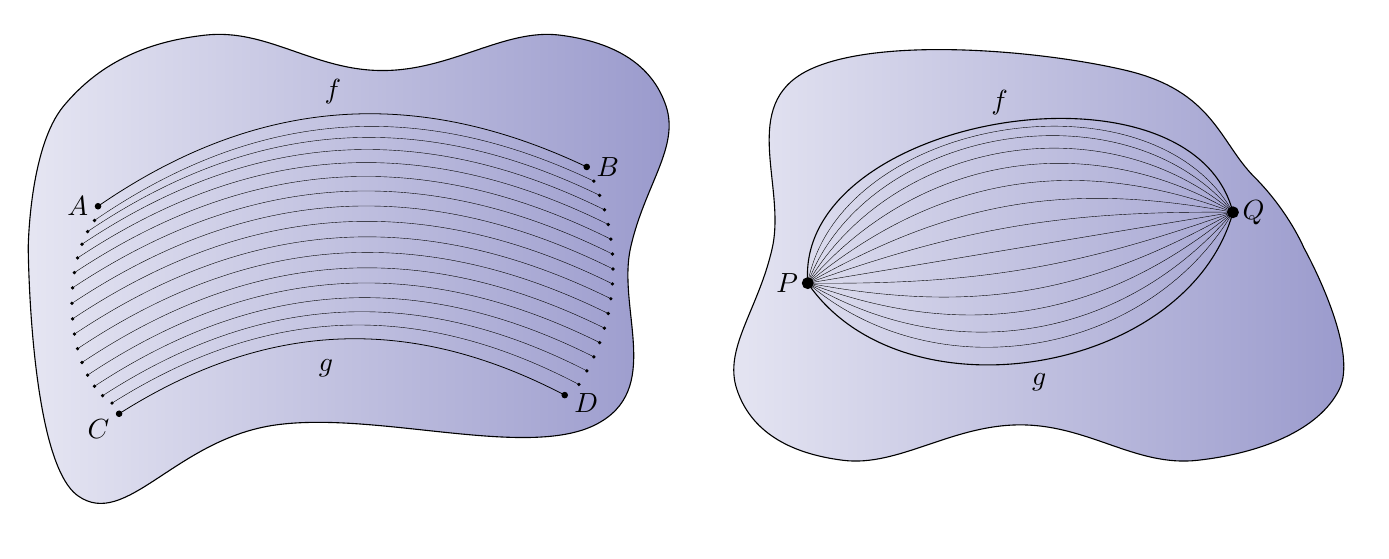
\begin{tikzpicture}[scale = 0.9]
\begin{scope}
\shade[draw, left color = NavyBlue!10, right color = NavyBlue!40] 
plot[smooth, tension=.7] coordinates {(-3.5,0.5)
(-3,2.5) (-1,3.5) (1.5,3) (4,3.5) (5.5,2.5) (5,.5) (4.5,-2)
(0,-2) (-2.8,-3) (-3.5,0.5)}; 

\begin{scope}[yshift = 1.2cm]
\coordinate (A) at (-2, 0.03);
\coordinate (a) at (-2, -3);

\coordinate (B) at (4, 1);
\coordinate (b) at (4, -3);

\foreach \t in {4, 5, ..., 18}{
\pgfmathsetmacro{\n}{\t*0.05}

\path (A) to[bend right = 85] coordinate[pos = \n] (A\t) (a);
\path (B) to[bend left = 40] coordinate[pos = \n] (B\t) (b);

\filldraw (A\t) circle (0.1ex);
\filldraw (B\t) circle (0.1ex) ;

\draw[line width = 0.05mm] (A\t) to[bend left] (B\t);
}

\draw[line width = 0.1mm] ([xshift = 0.1cm,  yshift=-0.15cm]A18) to[bend left] ([xshift = -0.2cm, yshift=-0.15cm]B18);
\draw[line width = 0.1mm] ([xshift = 0.05cm,  yshift=0.2cm]A4) to[bend left] ([xshift = -0.1cm, yshift=0.2cm]B4);


\filldraw ([xshift = 0.05cm,  yshift=0.2cm]A4) circle (0.25ex) node[left] {$A$};
\filldraw ([xshift = -0.1cm, yshift=0.2cm]B4) circle (0.25ex) node[right]{$B$};
\filldraw ([xshift = 0.1cm,  yshift=-0.15cm]A18) circle (0.25ex) node[left, yshift=-0.2cm] {$C$};
\filldraw ([xshift = -0.2cm, yshift=-0.15cm]B18) circle (0.25ex) node[right, yshift=-0.1cm] {$D$};
\end{scope}

\node at (0.8,2.7) {$f$};
\node at (0.7,-1.2) {$g$};
\end{scope}

\begin{scope}[xshift = 12cm, rotate = 180, yshift =-1cm]
\shade[draw, left color = NavyBlue!10, right color = NavyBlue!40] 
plot[smooth, tension=.7] coordinates {(-2.5,0.5)
(-3,2.5) (-1,3.5) (1.5,3) (4,3.5) (5.5,2.5) (5,.5) (4.5,-2)
(0,-2) (-1.8,-0.5) (-2.5,0.5)}; 

\begin{scope}[xshift = 2.5cm, yshift = 1cm, rotate = 180]
\coordinate (A) at (-2, 0);
\coordinate (B) at (4, 1);

\filldraw (A) circle (0.5ex) node[left]{$P$};
\filldraw (B) circle (0.5ex) node[right]{$Q$};

\foreach \p in {0,10,...,50}{
\draw[line width = 0.05mm] (A) to[bend right = \p] (B);
}
\foreach \p in {10,20,...,70}{
\draw[line width = 0.05mm] (A) to[bend left = \p] (B);
}
\draw (A) to[bend left = 85] coordinate (C) (B);
\node at ([yshift=0.3cm]C) {$f$};

\draw (A) to[bend right = 65] coordinate (D) (B);
\node at ([yshift=-0.3cm]D) {$g$};
\end{scope}
\end{scope}
\end{tikzpicture}
\end{center}